\documentclass[tikz,border=6pt]{standalone}
\usetikzlibrary{arrows.meta,positioning,calc,fit,backgrounds}
\newcommand{\NodeW}{30mm}
\definecolor{ink}{HTML}{1A1A1A}
\definecolor{rule}{HTML}{9AA3AB}
\definecolor{edge}{HTML}{555555}
\definecolor{tint}{HTML}{F7E9E9}
\definecolor{faint}{HTML}{C8CFD5}
\begin{document}
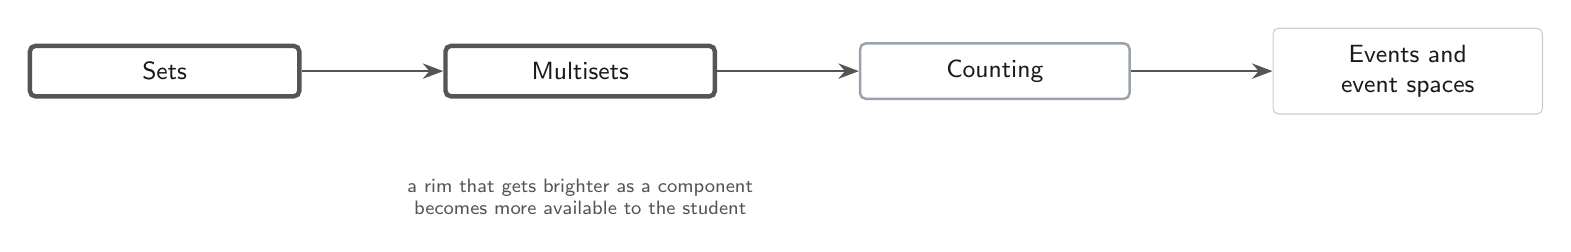
\begin{tikzpicture}[
  font=\sffamily\small,
  kc/.style={draw=rule, fill=white, rounded corners=2pt, text width=\NodeW,
             align=center, inner sep=6pt, text=ink},
  small/.style={draw=rule, fill=white, rounded corners=2pt, align=center,
                inner sep=4pt, text=ink, font=\sffamily\scriptsize},
  src/.style={draw=edge, fill=tint, circle, inner sep=5pt, text=ink,
              font=\sffamily\scriptsize, align=center},
  rel/.style={-{Stealth[length=2.6mm]}, draw=edge, thick},
  weak/.style={-{Stealth[length=2.6mm]}, draw=faint, thick, dashed},
  lab/.style={font=\sffamily\scriptsize, text=edge, align=center,
              fill=white, inner sep=2pt}
]
% rim brightness stands for how available a component has become
\tikzset{
  lit0/.style={kc, draw=faint},
  lit1/.style={kc, draw=rule, line width=0.9pt},
  lit2/.style={kc, draw=edge, line width=1.6pt}
}
\node[lit2] (sets) {Sets};
\node[lit2, right=18mm of sets] (multi) {Multisets};
\node[lit1, right=18mm of multi] (count) {Counting};
\node[lit0, right=18mm of count] (prob) {Events and\\event spaces};
\draw[rel] (sets) -- (multi);
\draw[rel] (multi) -- (count);
\draw[rel] (count) -- (prob);
\node[font=\sffamily\scriptsize, text=edge, align=center, below=9mm of multi]
  {a rim that gets brighter as a component\\becomes more available to the student};
\end{tikzpicture}
\end{document}
